\documentclass[10pt,x11names,table]{beamer}

\usetheme[progressbar=frametitle]{metropolis}
\usepackage{appendixnumberbeamer}
\usepackage{xcolor}

\usepackage{polyglossia}
\setmainlanguage{spanish}

\usepackage{listings}

\usepackage{booktabs}
\usepackage[scale=2]{ccicons}

\usepackage{pgfplots}
\usepgfplotslibrary{dateplot}

%ANIMACIONES
\usepackage{animate}
\usepackage{graphicx}
\usepackage[caption=false]{subfig}

\usepackage{xspace}

\newcommand*{\eg}{e.g.\@\xspace}
\newcommand*{\ie}{i.e.\@\xspace}

\let\oldquote\quote
\let\endoldquote\endquote
\renewenvironment{quote}[2][]
  {\if\relax\detokenize{#1}\relax
     \def\quoteauthor{#2}%
   \else
     \def\quoteauthor{#2~---~#1}%
   \fi
   \oldquote}
  {\par\nobreak\smallskip\hfill(\quoteauthor)%
   \endoldquote\addvspace{\bigskipamount}}
   
\usepackage{wrapfig}

\usepackage{subfig}
\usepackage{hyperref}
\usepackage{multicol}

\setbeamertemplate{bibliography item}[text]

\usepackage[font=small,skip=0pt, labelformat=empty]{caption}

\usepackage{dirtytalk}
\usepackage[acronym]{glossaries}
\makeglossaries

\newacronym{acgan}{ACGAN}{Auxiliary Classifier GAN}
\newacronym{ae}{AE}{Autoencoder}
\newacronym{ai}{AI}{Artificial Intelligence}
\newacronym{api}{API}{Application Programming Interface}
\newacronym{bert}{BERT}{Bidirectional Encoder Representations from Transformers}
\newacronym{brief}{BRIEF}{Binary Robust Independent Elementary Features}
\newacronym{brnn}{BRNN}{Bidirectional RNN}
\newacronym{bptt}{BPTT}{Backpropagation Through Time}
\newacronym{cbow}{CBOW}{Continous bag-of-words}
\newacronym{cnn}{CNN}{Convolutional Neural Network}
\newacronym{crnn}{CRNN}{Convolutional Recurrent Neural Network}
\newacronym{ddpm}{DDPM}{Denoising Diffusion Probabilistic Model}
\newacronym{ddim}{DDIM}{Denoising Diffusion Implicit Model}
\newacronym{diffit}{DiffiT}{Diffusion Vision Transformer}
\newacronym{dl}{DL}{Deep Learning}
\newacronym{dnn}{DNN}{Deep Neural Network}
\newacronym{dos}{DoS}{Denial of Service}
\newacronym{drnn}{DRNN}{Deep Recurrent Neural Network}
\newacronym{ecg}{ECG}{Electrocardiogram}
\newacronym{elmo}{ELMo}{Embedding from Language Model}
\newacronym{fast}{FAST}{Features from Accelerated Segment Test}
\newacronym{fid}{FID}{Fréchet Inception Distance}
\newacronym{foss}{FOSS}{Free and open-source software}
\newacronym{gan}{GAN}{Generative Adversarial Network}
\newacronym{glove}{GloVe}{Global Vectors for Word Representation}
\newacronym{gpu}{GPU}{Graphics Processing Unit}
\newacronym{gru}{GRU}{Gated Recurrent Unit}
\newacronym{ilsvrc}{ILSVRC}{ImageNet Large Scale Visual Recognition Challenge}
\newacronym{is}{IS}{Inception Score}
\newacronym{kid}{KID}{Kernel Inception Distance}
\newacronym{ldm}{LDM}{Latent Diffusion Model}
\newacronym{lstm}{LSTM}{Long Short-Term Memory}
\newacronym{mape}{MAPE}{Mean Absolute Perentage Error}
\newacronym{ml}{ML}{Machine Learning}
\newacronym{mlp}{MLP}{Multilayer Perceptron}
\newacronym{mmd}{MMD}{Maximum Mean Discrepancy}
\newacronym{mse}{MSE}{Mean Squared Error}
\newacronym{ner}{NER}{Named Entity Recognition}
\newacronym{nlg}{NLG}{Natural Language Generation}
\newacronym{nlp}{NLP}{Natural Language Processing}
\newacronym{nlu}{NLU}{Natural Language Understanding}
\newacronym{nn}{NN}{Neural Network}
\newacronym{ocr}{OCR}{Optical Character Recognition}
\newacronym{onnx}{ONNX}{Open Neural Network Exchange}
\newacronym{pmml}{PMML}{Predictive Model Markup Language}
\newacronym{relu}{ReLU}{Rectified Linear Unit}
\newacronym{rest}{REST}{Representational State Transfer}
\newacronym{rnn}{RNN}{Recurrent Neural Network}
\newacronym{sae}{SAE}{Stacked Autoencoder}
\newacronym{sift}{SIFT}{Scale-Invariant Feature Transform}
\newacronym{slam}{SLAM}{Simultaneous Localization and Mapping}
\newacronym{sru}{SRU}{Single Recurrent Unit}
\newacronym{surf}{SURF}{Speeded-Up Robust Features}
\newacronym{svm}{SVM}{Support Vector Machine}
\newacronym{vae}{VAE}{Variational Autoencoder}
\newacronym{vgg}{VGG}{Visual Geometry Group}
\newacronym{vit}{ViT}{Vision Transformer}
\newacronym{wsgi}{WSGI}{Web Server Gateway Interface}
\newacronym{xai}{XAI}{eXplainable Artificial Intelligence}
\newacronym{yolo}{YOLO}{You Only Look Once}
\newacronym{zsl}{ZSL}{Zero-shot Learning}
\subtitle{Métodos Generativos, curso 2024-2025}

\date{\today}
\author{Guillermo Iglesias, guillermo.iglesias@upm.es \newline
Jorge Dueñas Lerín, jorge.duenas.lerin@upm.es  \newline
Félix Fuentes Hurtado, felix.fuentes@upm.es}

\institute{Escuela Técnica Superior de Ingeniería de Sistemas Informáticos | UPM \newline
\hbox{} \newline \ccbysa \hspace{0.1pt} \ccNonCommercial}

%%%%%%%%%%%%%%%%%%%%%%%%%%%%%%%%%%%%%       
\title{Variational Autoencoders}

\begin{document}
\maketitle

\begin{frame}{Contenidos}
  \begin{enumerate}
      \item Introducción
      \item Auto-encoders (AEs)
      \item{Auto-encoders Variacionales (VAEs)}
      \item{Generative Adversarial Networks (GANs)}
      \item{Transformers}
      \item{Diffusion Models}
    \end{enumerate}
\end{frame}


\begin{frame}{Contenidos}
  \begin{enumerate}
      \item Introducción
      \item Auto-encoders (AEs)
      \item{\textbf{Auto-encoders Variacionales (VAEs)}}
      \item{Generative Adversarial Networks (GANs)}
      \item{Transformers}
      \item{Diffusion Models}
    \end{enumerate}
\end{frame}

\section{Auto-encoders Variacionales (VAEs)}

\begin{frame}{Motivación}

Los autoencoders tienen un gran problema: no son buenos \textbf{generadores} de datos.
\newline
\newline
\centering\textbf{¿Por qué?}
\end{frame}

\begin{frame}{Motivación}

Pensemos en un ejemplo sencillo: la reconstrucción de imágenes del dataset MNIST.

¿Cómo pensáis que será el espacio latente (representación en el \textit{bottleneck})?

\end{frame}

\begin{frame}{Motivación}

\begin{figure}
    \centering
    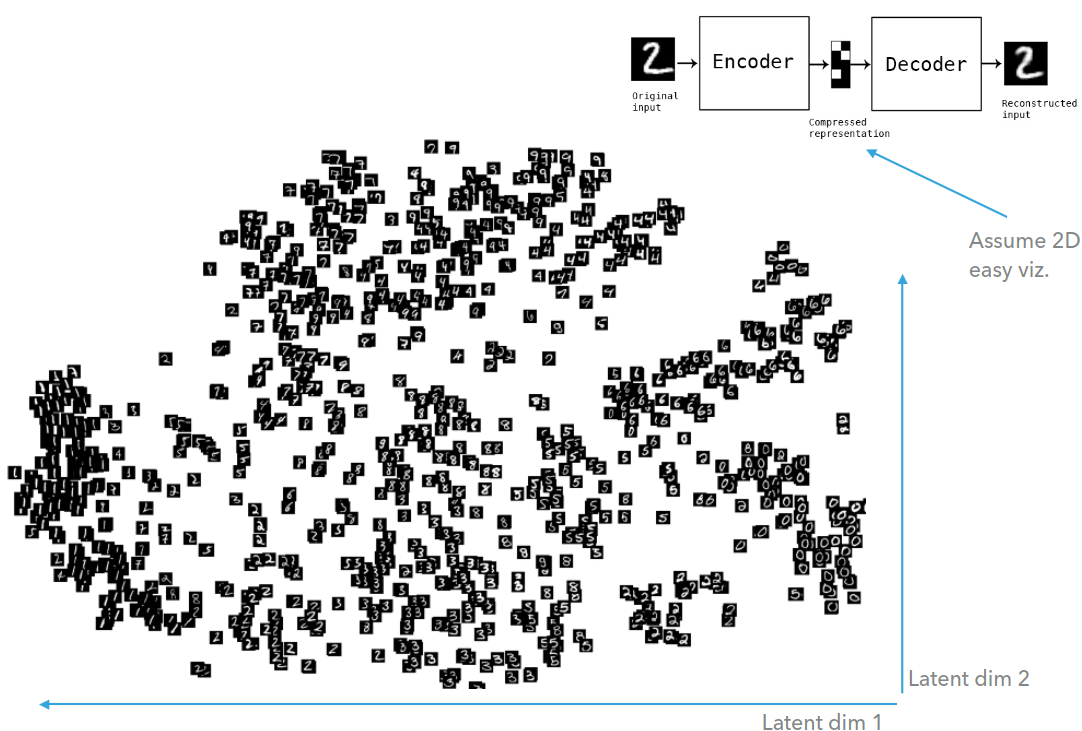
\includegraphics[width=0.7\textwidth]{Slides/figures/02_Metodos_Generativos/ae-latent-space.png}
    \caption{Ejemplo de espacio latente con el dataset MNIST (\href{https://indico.ictp.it/event/8674/session/155/contribution/1121/material/slides/0.pdf}{fuente}).}
    \label{fig:enter-label}
\end{figure}

\end{frame}

\begin{frame}{Motivación}

Esta representación presenta determinados problemas: al no ser continua, tendremos problemas cuando la entrada sea ligeramente distinta a los datos con los que se entrenó el autoencoder:

¿Qué ocurrirá cuando la entrada sean imágenes que generen códigos latentes entre medio de las muestras de entrenamiento?

\begin{figure}
    \centering
    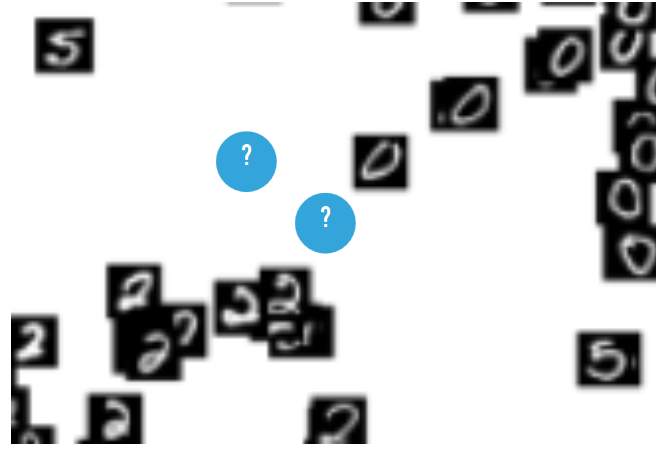
\includegraphics[width=0.4\textwidth]{Slides/figures/02_Metodos_Generativos/ae-zoom-latent-space.png}
    \caption{Ejemplo de problemas al generar nuevas muestras (\href{https://indico.ictp.it/event/8674/session/155/contribution/1121/material/slides/0.pdf}{fuente}).}
    \label{fig:enter-label}
\end{figure}

\end{frame}


\begin{frame}{Motivación}

Esta imagen lo muestra de forma intuitiva:

\begin{figure}
    \centering
    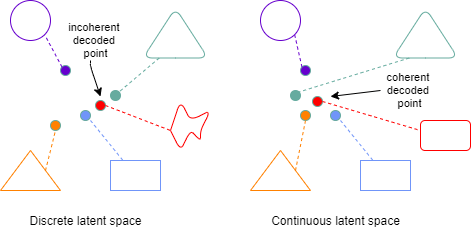
\includegraphics[width=0.8\textwidth]{Slides/figures/02_Metodos_Generativos/ae vs vae sampling.png}
    \caption{Ejemplo de problemas al generar \textit{muestrear} de un espacio latente no continuo (\href{https://www.researchgate.net/publication/349939162/figure/fig1/AS:999624672305152@1615340502225/Simplified-representation-of-the-compression-resulting-from-a-vanilla-Autoencoder-left.ppm}{fuente}).}
    \label{fig:enter-label}
\end{figure}

\end{frame}


\begin{frame}{Motivación}

¿Qué es lo deseable?

\begin{itemize}
    \item Un espacio latente \textbf{continuo} y \textbf{ordenado}
    \item en el que poder obtener muestras parecidas a los datos de la entrada aunque no coincidan exactamente con alguno de los de entrenamiento
    \item y en el que poder \textbf{interpolar} entre distintos espacios latentes para obtener \textbf{nuevas muestras}
\end{itemize}

\begin{figure}
    \centering
    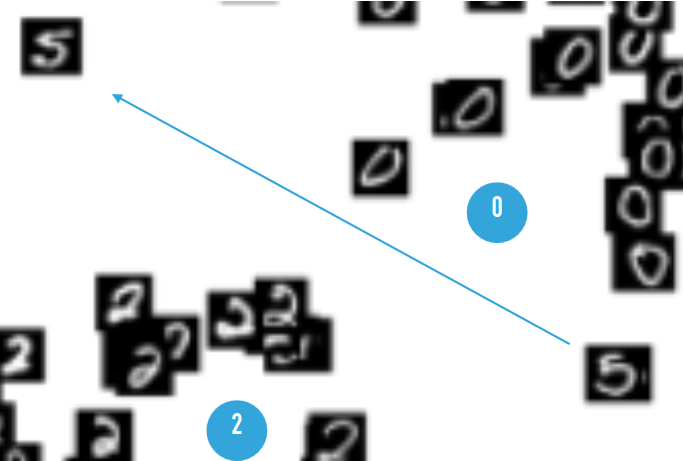
\includegraphics[width=0.38\textwidth]{Slides/figures/02_Metodos_Generativos/ae-desired-latent-space.png}
    \caption{Ejemplo de problemas al generar nuevas muestras (\href{https://indico.ictp.it/event/8674/session/155/contribution/1121/material/slides/0.pdf}{fuente}).}
    \label{fig:enter-label}
\end{figure}

\end{frame}


\begin{frame}{Motivación}

Ejemplo de interpolación con un espacio latente \textbf{contínuo} y \textbf{ordenado}:

\begin{figure}
    \centering
    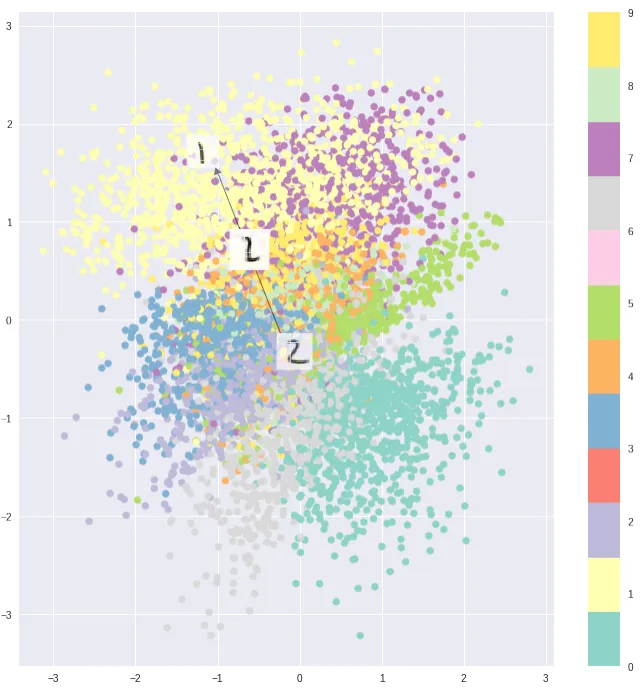
\includegraphics[width=0.4\textwidth]{Slides/figures/02_Metodos_Generativos/vae-interpolation.png}
    \caption{Ejemplo de interpolación (\href{https://towardsdatascience.com/intuitively-understanding-variational-autoencoders-1bfe67eb5daf}{fuente}).}
    \label{fig:enter-label}
\end{figure}

\end{frame}


\begin{frame}{Motivación}

\textbf{¿Cómo lo logramos?}

Modificando ligeramente la arquitectura del auto-encoder para conseguir un espacio latente \textbf{contínuo} y \textbf{ordenado}.

\begin{figure}
    \centering
    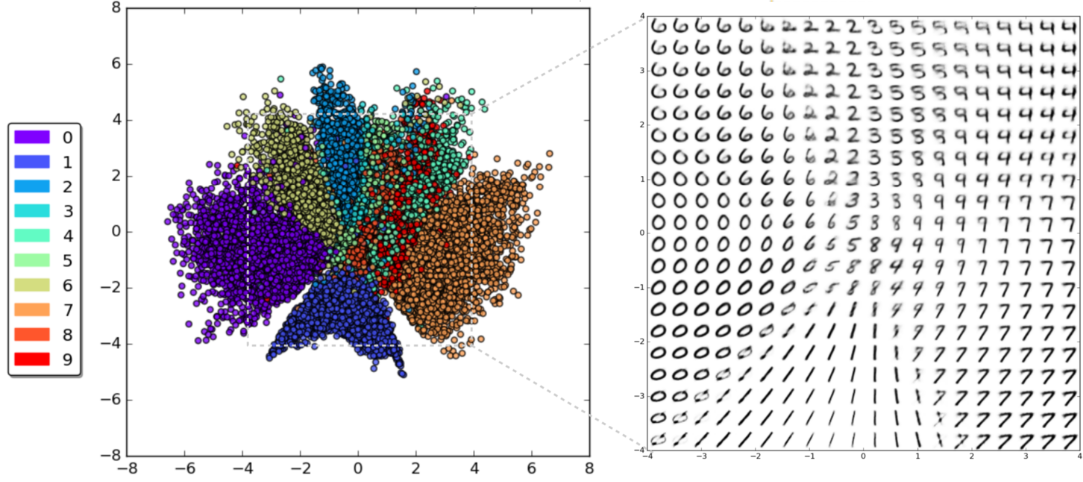
\includegraphics[width=0.7\textwidth]{Slides/figures/02_Metodos_Generativos/vae-continuous-latent-space.png}
    \caption{Ejemplo de espacio latente \textbf{contínuo} y \textbf{ordenado} de las muestras generadas a partir de su muestreo. (\href{https://indico.ictp.it/event/8674/session/155/contribution/1121/material/slides/0.pdf}{fuente}).}
    \label{fig:enter-label}
\end{figure}

\end{frame}

\begin{frame}{\acrfullpl{vae}}

\textbf{¿Qué son los Auto-Encoders Variacionales (VAEs)?}
Son una variante de los autoencoders~\cite{kingma2019introduction} que permiten la generación de datos sintéticos.

\begin{itemize}
    \item Combinan redes neuronales con distribuciones de probabilidad.
    \item Permiten que los datos generados sigan el mismo patrón que los datos de entrada.
\end{itemize}

Así, la red aprende los parámetros de una distribución de probabilidad.

\begin{itemize}
    \item Construyen explícitamente un \textbf{espacio latente continuo} y \textbf{ordenado}.
    \item No una función arbitraria como en las redes neuronales convencionales.
\end{itemize}
\end{frame}

\begin{frame}{¿Cómo funcionan?}
En los \glspl{vae}, el espacio latente está definido por \textbf{dos vectores de tamaño $n$}:

\begin{itemize}
    \item $\vec{\mu} = (\mu_1, \ldots, \mu_n)$: Vector de \textbf{medias}.
    \item $\vec{\sigma} = (\sigma_1, \ldots, \sigma_n)$: Vector de \textbf{desviaciones estándar}.
\end{itemize}

Forman un vector de distribuciones normales: $(N(\mu_1,\sigma_1),\ldots ,N(\mu_n,\sigma_n))$.

\begin{itemize}
    \item Cada $\mu_i$ controlará el centro aproximado donde codificar los datos de entrada.
    \item Cada $\sigma_i$ controlará cuánto pueden desviarse en cualquiera de sus muestras.
\end{itemize}

Con este modelo, el decodificador asocia áreas completas (no solo puntos individuales) a variantes ligeras de la misma salida.

\begin{itemize}
    \item Esto resulta en un espacio interpolado mucho más suave.
    \item Es capaz de producir nuevas salidas que comparten propiedades.
\end{itemize}
\end{frame}

\begin{frame}{Estructura}
El espacio latente está definido por \textbf{dos vectores de tamaño $n$}:

\begin{center}
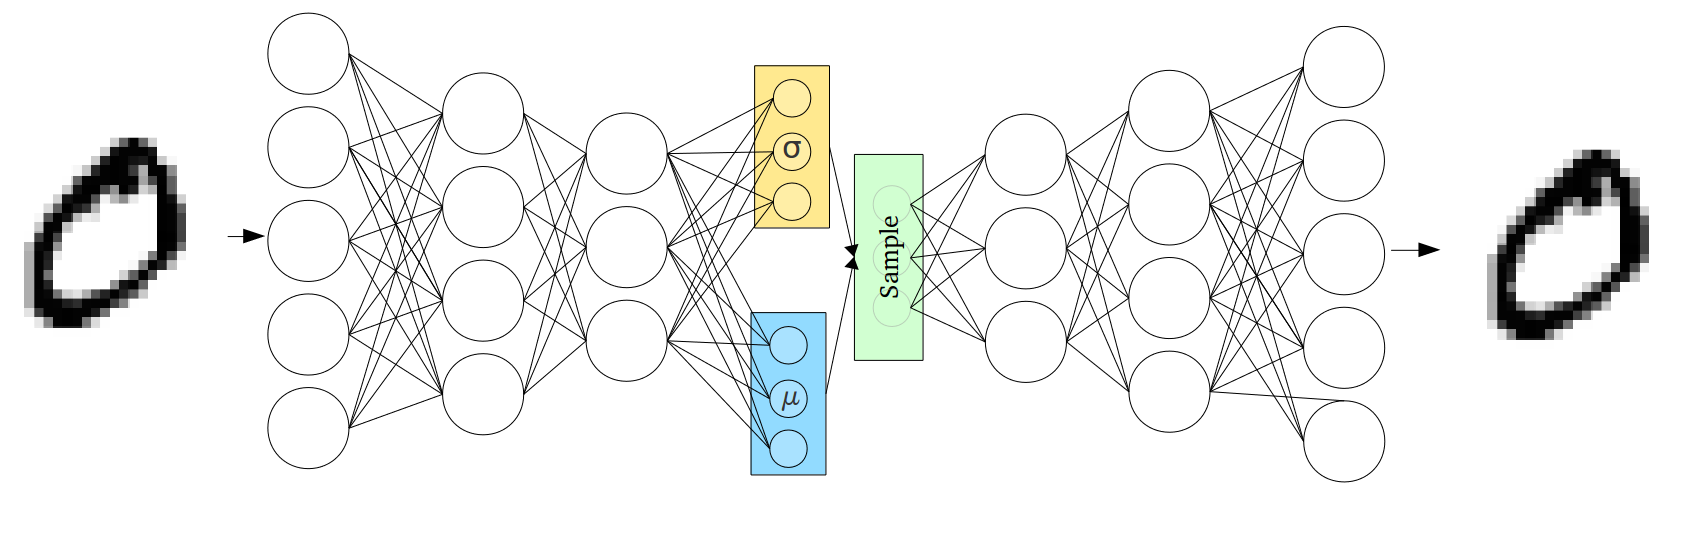
\includegraphics[width=.8\textwidth]{Slides/figures/02_Metodos_Generativos/nn-vae.png}
\end{center}

Luego debemos ajustar las funciones de pérdida individualmente de tal manera que:

\begin{itemize}
    \item Una \textbf{función de pérdida tradicional} que calcula la \textbf{diferencia} con el objeto generado.
    \item La \textbf{divergencia KL (Kullback-Leibler)} entre la distribución latente aprendida y la distribución anterior (\textit{prior distribution}), que actúa como término de regularización. 
    \item Se suele usar $\mathcal{N}(0, 1)$
\end{itemize}
\end{frame}

\begin{frame}{Estructura}

\textbf{¿Por qué necesitamos las pérdidas de reconstrucción y la divergencia KL?}


\begin{figure}
    \centering
    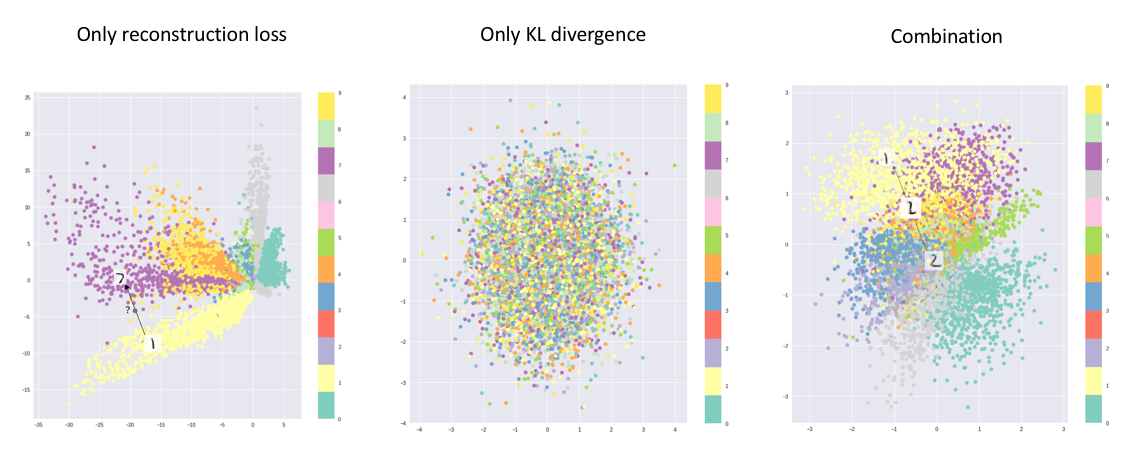
\includegraphics[width=1\textwidth]{Slides/figures/02_Metodos_Generativos/vae-comparison-mse-and-kl.png}
    \caption{Ejemplo con diferentes términos de la función de pérdidas (\href{https://www.jeremyjordan.me/content/images/2018/03/Screen-Shot-2018-03-18-at-7.22.24-PM.png}{fuente}).}
    \label{fig:enter-label}
\end{figure}

\end{frame}

\begin{frame}{Divergencia KL (I)}
Mide la diferencia entre dos distribuciones de probabilidad.

\begin{center}
    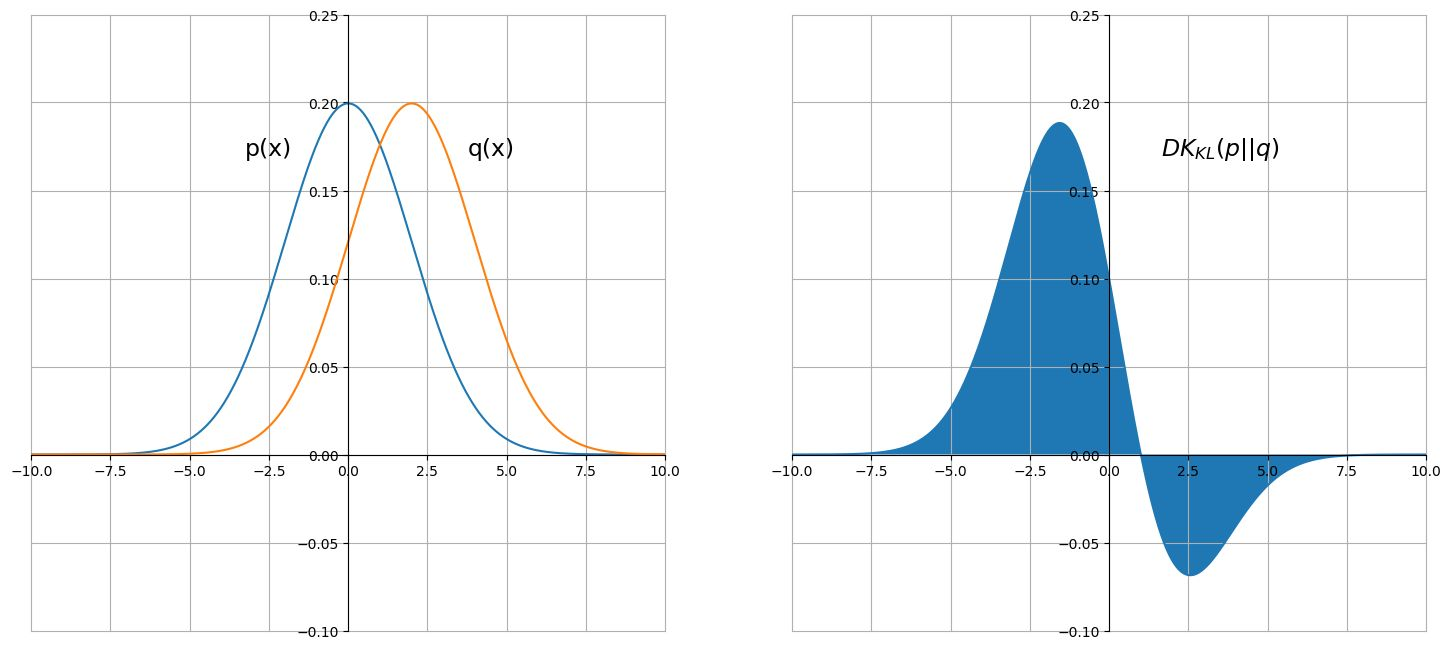
\includegraphics[width=.6\textwidth]{Slides/figures/02_Metodos_Generativos/nn-kl-divergence.png}
\end{center}

Por ejemplo, en las distribuciones de la figura tenemos dos distribuciones:

\begin{itemize}
    \item Una distribución normal y conocida $p(x)$.
    \item Una distribución normal y desconocida $q(x)$.
\end{itemize}

Es una \textbf{divergencia, no una distancia}, ya que no es simétrica.
\end{frame}

\begin{frame}{Divergencia KL (II)}
Forzando una distribución normal estándar ($\mu = 0$ y $\sigma = 1$) para nuestra distribución de datos, tenemos que la divergencia KL se puede calcular como:

$$
KL = \sum_{i=1}^{n}\sigma_{i}^{2} + \mu_{i}^{2}-log(\sigma_i)-1
$$

Nuestra función de pérdida consistirá en dos términos:

\begin{itemize}
    \item Función de pérdida tradicional $\mathcal{L}_r$: Ajustará los datos de salida.
    \item Función de divergencia $KL$: Ajustará el espacio latente a la distribución estándar.
\end{itemize}

Por lo tanto, la expresión de la función de pérdida será:

$$
\mathcal{L}(y, \hat{y}) = \mathcal{L}_r(y, \hat{y}) + \mathcal{L}_{\text{KL}} (y, \hat{y})
$$

\end{frame}

\begin{frame}{Aplicaciones}

Una aplicación de los VAEs es la de poder generar muestras teniendo \alert{cierto} control sobre lo que generamos.

\begin{figure}
    \centering
    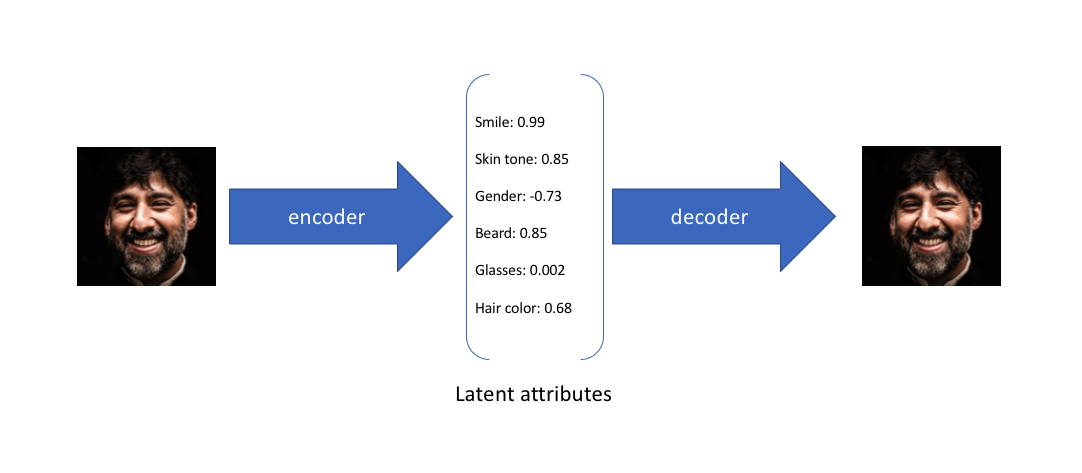
\includegraphics[width=.7\textwidth]{Slides/figures/02_Metodos_Generativos/vae-face-generator.png}
    \caption{Ejemplo de generación de caras controlando los atributos (\href{https://www.jeremyjordan.me/variational-autoencoders/}{fuente}).}
    \label{fig:enter-label}
\end{figure}

En los VAEs el espacio latente está \alert{entrelazado}. \href{https://github.com/nnormandin/Conditional_VAE/blob/master/Conditional_VAE.ipynb}{Conditional VAE}. Se verá en CGANs.
    
\end{frame}

\begin{frame}{Aplicaciones}

¿Cómo se comportarían un AE y un VAE a la hora de caracterizar la sonrisa de una imagen?

\begin{figure}
    \centering
    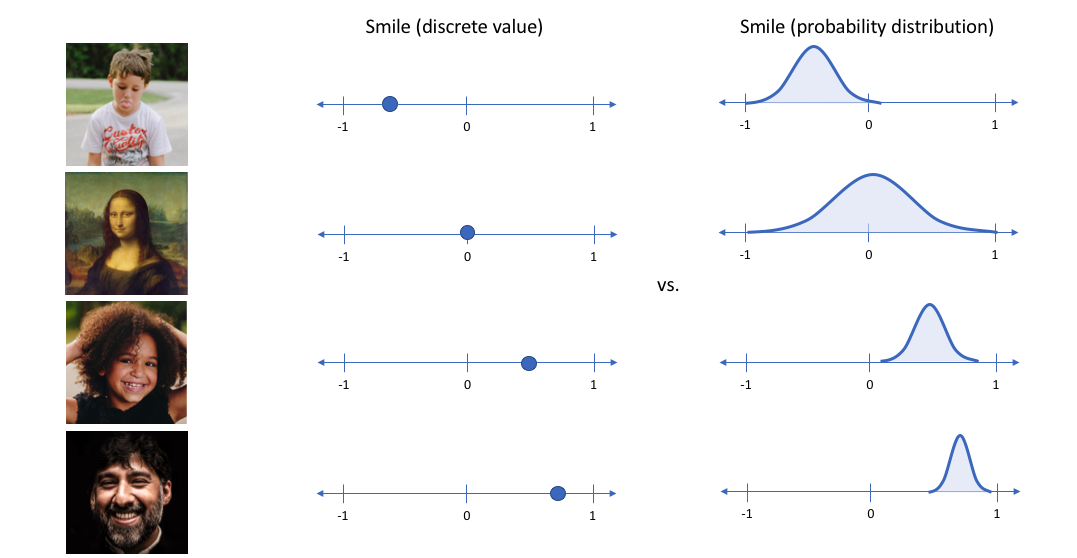
\includegraphics[width=.7\textwidth]{Slides/figures/02_Metodos_Generativos/vae-face-generator-smile.png}
    \caption{Ejemplo de espacio latente en AEs vs VAEs (\href{https://www.jeremyjordan.me/variational-autoencoders/}{fuente}).}
    \label{fig:enter-label}
\end{figure}
    
\end{frame}

\iffalse

\begin{frame}{Aplicaciones}

Con los VAEs podemos conseguir asignar una distribución de probabilidad a cada característica que queremos controlar, dándonos capacidad de "jugar" con ellas:

\begin{figure}
    \centering
    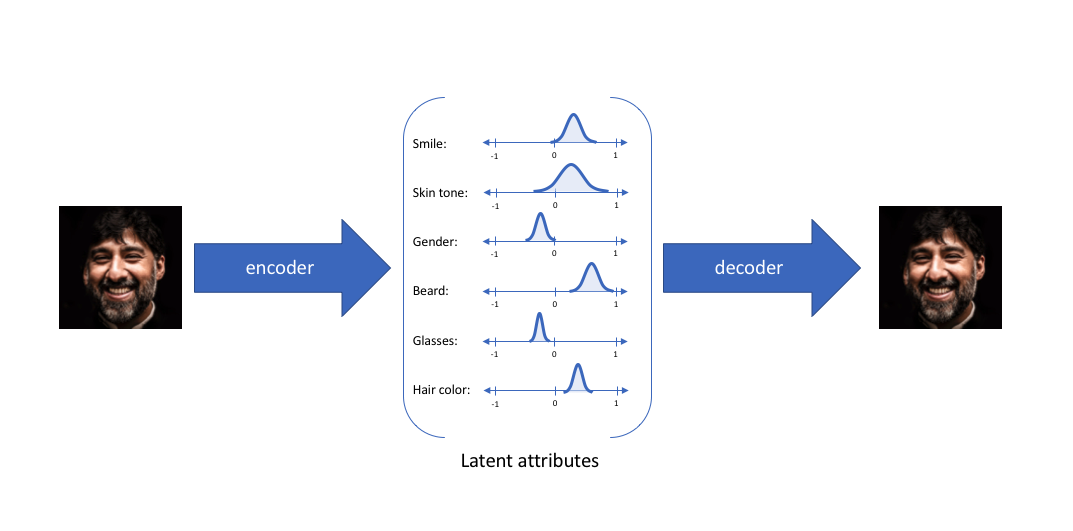
\includegraphics[width=.8\textwidth]{Slides/figures/02_Metodos_Generativos/vae-face-generator-smile_pds.png}
    \caption{Ejemplo de generación de caras controlando los atributos (\href{https://www.jeremyjordan.me/variational-autoencoders/}{fuente}).}
    \label{fig:enter-label}
\end{figure}
    
\end{frame}

\fi

\begin{frame}{Aplicaciones}

Al contrario que con los AEs, con los VAEs podemos obtener muestras nuevas diferentes a las de entrenamiento.

Por ejemplo, si muestreamos dos veces con valores similares, deberemos obtener muestras similares:

\begin{figure}
    \centering
    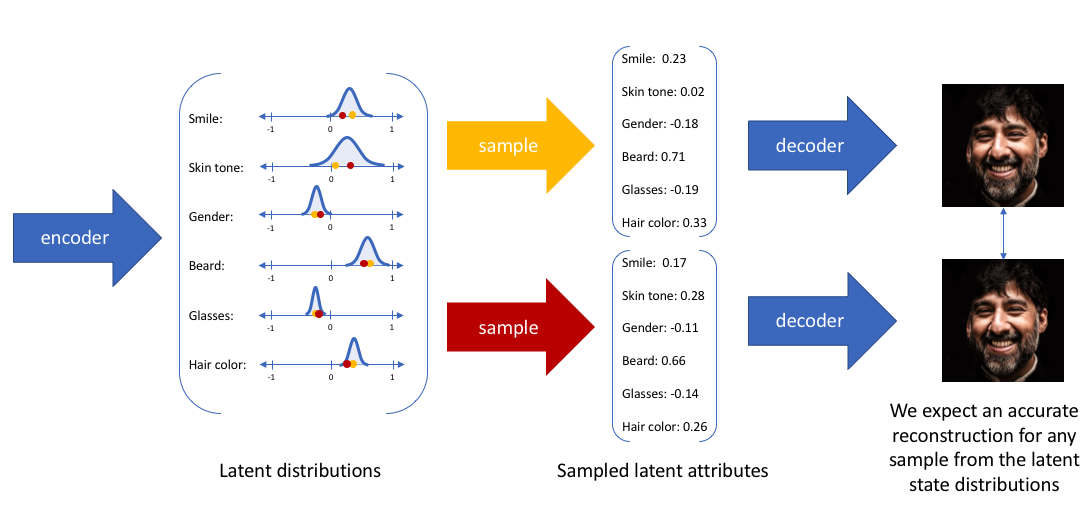
\includegraphics[width=.7\textwidth]{Slides/figures/02_Metodos_Generativos/vae-face-generator-smile_pds-example.png}
    \caption{Ejemplo de generación de dos caras similares controlando los atributos (\href{https://www.jeremyjordan.me/variational-autoencoders/}{fuente}).}
    \label{fig:enter-label}
\end{figure}
    
\end{frame}


\begin{frame}{Bonus: ¿Aprendizaje supervisado o no supervisado?}

Tradicionalmente, se han clasificado como \textbf{aprendizaje no supervisado}.

\begin{itemize}
    \item Después de todo, no trabajan con datos etiquetados.
    \item ¡Pero no puedes optimizar autoencoders sin la retroalimentación de la propia reconstrucción!
\end{itemize}

En el \textbf{aprendizaje supervisado}, se aprende con retroalimentación de los datos.

\begin{itemize}
    \item Se espera que, al proporcionar algunos ejemplos, el algoritmo descubra la función que mapea las entradas a las salidas deseadas con el menor error.
\end{itemize}

Yann LeCun inventó el término \textbf{aprendizaje auto-supervisado} para hablar sobre estos modelos.
\end{frame}

\begin{frame}

{\Large\it I now call it ``self-supervised learning'', because ``unsupervised'' is both a loaded and confusing term. [\ldots] Self-supervised learning uses way more supervisory signals than supervised learning, and enormously more than reinforcement learning. That's why calling it ``unsupervised'' is totally misleading.}

\begin{flushright}
Yann LeCun - Recent Advances in Deep Learning (2019)
\end{flushright}
\end{frame}

\begin{exercise}
\href{https://colab.research.google.com/drive/11KvEtZmi33OrZVFO9uP9d68-nQrwfO-9}{Generación de imágenes con \acrlongpl{vae}}
\end{exercise}

%%%%%%%%%%%%%%%%%%%%%%%%%%%%

\begin{frame}{Recursos}
\begin{itemize}
    \item Diapositivas de Moodle
    \item Google Collaboratory
    \item Deep Learning Book (https://www.deeplearningbook.org/)
    \item https://www.pyimagesearch.com/blog
    \item https://machinelearningmastery.com/blog
\end{itemize}
\end{frame}


% \section{Generative Adversarial Networks (GANs)}
% % \begin{frame}{Generative Adversarial Networks (GANs)}
% % \end{frame}

% \section{Transformers}
% % \begin{frame}{Transformers}
% % \end{frame}

% \section{Diffusion Models}
% % \begin{frame}{Diffusion Models}
% % \end{frame}


\appendix

\begin{frame}[allowframebreaks]{Referencias}
    \bibliography{references}
    \bibliographystyle{abbrv}
\end{frame}

\begin{frame}<presentation:0>{License}
    \begin{block}{Tema \texttt{slides-upm}. Puedes obtener sus fuentes en}
        \begin{center}\url{http://gitlab.com/blazaid/slides-upm}\end{center}
    \end{block}
  
    Tanto esta presentación como el tema están licenciados bajo \href{http://creativecommons.org/licenses/by-sa/4.0/}{Creative Commons
  Atribución-CompartirIgual 4.0 Internacional (CC BY-SA 4.0)}.
    \begin{center}\ccbysa\end{center}
\end{frame}

\end{document}
